%% Copyright (c) 2023, RTE (http://www.rte-france.com)
%% See AUTHORS.txt
%% All rights reserved.
%% This Source Code Form is subject to the terms of the Mozilla Public
%% License, v. 2.0. If a copy of the MPL was not distributed with this
%% file, you can obtain one at http://mozilla.org/MPL/2.0/.
%% SPDX-License-Identifier: MPL-2.0
%%
%% This file is part of Dynawo, an hybrid C++/Modelica open source suite
%% of simulation tools for power systems.

\documentclass[a4paper, 12pt]{report}

%% Except where otherwise noted, content in this documentation is Copyright (c)
%% 2015-2019, RTE (http://www.rte-france.com) and licensed under a
%% CC-BY-4.0 (https://creativecommons.org/licenses/by/4.0/)
%% license. All rights reserved.

% Latin Modern fam­ily of fonts
\usepackage{lmodern}

\usepackage[english]{babel}

% specify encoding
\usepackage[utf8]{inputenc} % input
\usepackage[T1]{fontenc} % output

% Document structure setup
\usepackage{titlesec} % To change chapter format
\setcounter{tocdepth}{3} % Add subsubsection in Content
\setcounter{secnumdepth}{3} % Add numbering for subsubsection
\setlength{\parindent}{0pt} % No paragraph indentation

% Change title format for chapter
\titleformat{\chapter}{\Huge\bf}{\thechapter}{20pt}{\Huge\bf}

% To add links on page number in Content and hide red rectangle on links
\usepackage[hidelinks, linktoc=all]{hyperref}
\usepackage[nottoc]{tocbibind}  % To add biblio in table of content
\usepackage{textcomp} % For single quote
\usepackage{url} % Allow linebreaks in \url command
\usepackage{listings} % To add code samples

% Default listings parameters
\lstset
{
  aboveskip={1\baselineskip}, % a bit of space above
  backgroundcolor=\color{shadecolor}, % choose the background color
  basicstyle={\ttfamily\footnotesize}, % use font and smaller size \small \footnotesize
  breakatwhitespace=true, % sets if automatic breaks should only happen at whitespace
  breaklines=true, % sets automatic line breaking
  columns=fixed, % nice spacing -> fixed / flexible
  mathescape=false, % escape to latex false
  numbers=left, % where to put the line-numbers
  numberstyle=\tiny\color{gray}, % the style that is used for the line-numbers
  showstringspaces=false, % do not emphasize spaces in strings
  tabsize=4, % number of spaces of a TAB
  texcl=false, % activates or deactivates LaTeX comment lines
  upquote=true % upright quotes
}

% Avoid numbering starting at each chapter for figures
\usepackage{chngcntr}
\counterwithout{figure}{chapter}

\usepackage{tikz} % macro pack­age for cre­at­ing graph­ics
\usepackage{pgfplots} % draws func­tion plots (based on pgf/tikz)

\usepackage{algorithm} % Add algorithms
\usepackage[noend]{algpseudocode} %  all end ... lines are omitted in algos

\usepackage{amsmath} % Add math­e­mat­i­cal fea­tures
\usepackage{schemabloc} % Add block diagram library (french one)

\usepackage{adjustbox} % Add box for flowchart

\usepackage{booktabs} % for toprule and midrule in tables

\usepackage{tabularx}

\usepackage[nolist]{acronym} % don’t write the list of acronyms.
% Acronyms list
\begin{acronym}
\acro{BDF}{Backward Differentiation Formula}
\acro{BE}{Backward Euler}
\acro{DAE}{Differential Algebraic Equations}
\acro{IDA}{Implicit Differential-Algebraic solver}
\acro{LLNL}{Lawrence Livermore National Lab}
\acro{KINSOL}{Krylov Inexact Newton SOLver}
\acro{NR}{Newton-Raphson}
\acro{PLL}{Phase-Locked Loop}
\acro{SVC}{Static Var Compensator}
\acro{SUNDIALS}{SUite of Nonlinear and DIfferential/ALgebraic equation Solvers}
\acro{WECC}{Western Electricity Coordinating Council}
\end{acronym}

% Syntax highlight
%% Except where otherwise noted, content in this documentation is Copyright (c)
%% 2015-2019, RTE (http://www.rte-france.com) and licensed under a
%% CC-BY-4.0 (https://creativecommons.org/licenses/by/4.0/)
%% license. All rights reserved.

\usepackage{color}

\definecolor{blue}{rgb}{0,0,1}
\definecolor{lightblue}{rgb}{.3,.5,1}
\definecolor{darkblue}{rgb}{0,0,.4}
\definecolor{red}{rgb}{1,0,0}
\definecolor{darkred}{rgb}{.56,0,0}
\definecolor{pink}{rgb}{.933,0,.933}
\definecolor{purple}{rgb}{0.58,0,0.82}
\definecolor{green}{rgb}{0.133,0.545,0.133}
\definecolor{darkgreen}{rgb}{0,.4,0}
\definecolor{gray}{rgb}{.3,.3,.3}
\definecolor{darkgray}{rgb}{.2,.2,.2}
\definecolor{shadecolor}{gray}{0.925}

% **********************************************************************************
% Syntax : Bash (bash)
% **********************************************************************************

\lstdefinelanguage{bash}
{
  keywordstyle=\color{blue},
  morekeywords={
    cd,
    export,
    source},
  numbers=none,
  deletekeywords={jobs}
}

% **********************************************************************************
% Syntax : XML
% **********************************************************************************

\lstdefinelanguage{XML}
{
  morestring=[s][\color{purple}]{"}{"},
  morecomment=[s][\color{green}]{<?}{?>},
  morecomment=[s][\color{green}]{<!--}{-->},
  stringstyle=\color{black},
  identifierstyle=\color{blue},
  keywordstyle=\color{red},
  morekeywords={
    xmlns,
    xsi,
    noNamespaceSchemaLocation,
    type,
    source,
    target,
    version,
    tool,
    transRef,
    roleRef,
    objective,
    eventually}
}

% **********************************************************************************
% Syntax : Modelica (modelica)
% **********************************************************************************
\lstdefinelanguage{Modelica}{
  alsoletter={...},
  morekeywords=[1]{ % types
      Boolean,
      Integer,
      Real},
  keywordstyle=[1]\color{red},
  morekeywords=[2]{ % keywords
    algorithm,
    and,
    annotation,
    assert,
    block,
    class,
    connector,
    constant,
    discrete,
    else,
    elseif,
    elsewhen,
    end,
    equation,
    exit,
    extends,
    external,
    false,
    final,
    flow,
    for,
    function,
    if,
    in,
    inner,
    input,
    import,
    loop,
    model,
    nondiscrete,
    not,
    or,
    outer,
    output,
    package,
    parameter,
    public,
    protected,
    record,
    redeclare,
    replaceable,
    return,
    size,
    terminate,
    then,
    true,
    type,
    when,
    while},
  keywordstyle=[2]\color{darkred},
  morekeywords=[3]{ % functions
    abs,
    acos,
    asin,
    atan,
    atan2,
    Complex,
    connect,
    conj,
    cos,
    cosh,
    cross,
    der,
    edge,
    exp,
    fromPolar,
    imag,
    noEvent,
    pre,
    sign,
    sin,
    sinh,
    sqrt,
    tan,
    tanh},
  keywordstyle=[3]\color{blue},
  morecomment=[l][\color{green}]{//}, % comments
  morecomment=[s][\color{green}]{/*}{*/}, % comments
  morestring=[b][\color{pink}]{'}, % strings
  morestring=[b][\color{pink}]{"}, % strings
}


\usepackage{xspace} % Define typography
\usepackage{dirtree}
\newcommand{\Dynawo}[0]{Dyna$\omega$o\xspace}


\begin{document}

\title{IEEE30 bus system}

\maketitle

\chapter*{Test case description}

The IEEE 30 bus system test case has 30 buses, 6 generators, 2 shunts, 4 transformers, 37 lines
and 21 loads. There are three voltage levels in the test case: 132 kV, 33 kV and 11 kV. The lower
outer part of the system with generators 1, 2, 5, 7 corresponds to the 132 kV network.

\begin{figure}[H]
  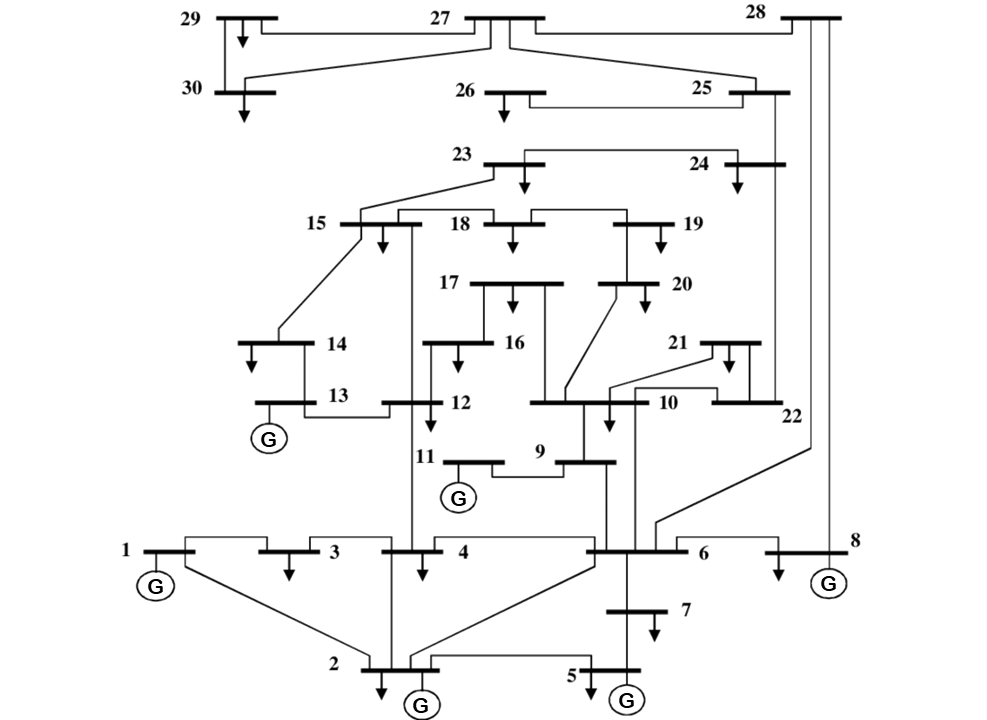
\includegraphics[scale=0.5]{IEEE30BusSystem.png}
  \caption{IEEE30 bus system diagram}
\end{figure}

\section{Initial conditions}

The reference angle for the load flow is set at bus n°1. The initial conditions for each generator
are: \\

\begin{tabular}{ | m{2cm} | m{2cm}| m{2cm} | m{2cm} | m{2cm} | }
  \hline
  \textbf{Generator} & \textbf{P (MW)} & \textbf{Q (Mvar)} & \textbf{U (kV)} & \textbf{$\Theta$ (°)} \\
  \hline
  1 & 260.95 & -16.79 & 139.20 & 0.00 \\
  \hline
  2 & 40.00 & 50.00 & 137.94 & -5.35 \\
  \hline
  5 & 0.00 & 36.85 & 133.32 & -14.16 \\
  \hline
  8 & 0.00 & 37.14 & 133.32 & -11.81 \\
  \hline
  11 & 0.00 & 16.17 & 11.90 & -14.11 \\
  \hline
  13 & 0.00 & 10.62 & 11.78 & -14.93 \\
  \hline
\end{tabular} \\

\section{Scenarios}

The following scenarios are presented based on the DynaSwing, DynaFlow and DynaWaltz documentation : \\

1) Three-phase fault \\
2) Disconnection of a line \\
3) Generator disconnection

\chapter{Scenario 1 : Three-phase fault at bus 2}

The simulated scenario is three-phase fault (R = 10e-4 $\Omega$, X = 10e-4 $\Omega$) at bus 2, which corresponds
to the point of connection for generator 2. The fault lasts from 1 to 1.1 s.

\section{Models}

\begin{itemize}
  \item Generators : four windings synchronous generators with a proportional voltage regulator and a proportional speed governor. Saturations are considered.
  \item Frequency model: explicit frequency model OmegaRef using different generator speeds
  \item Loads: alpha-beta load
\end{itemize}

\section{Solver}

IDA : order 2, absolute accuracy $10^{-4}$, relative accuracy $10^{-4}$.

\section{Results}

The response at bus 2 is analyzed. The voltage at node 2 falls to zero and consequently the active
power too. After the fault is cleared, both are stabilized. The machines dynamic data and the
explicit frequency model parameters should be adapted to achieve the desired response.

\begin{figure}[H]
  \centering
    \subfigure[]{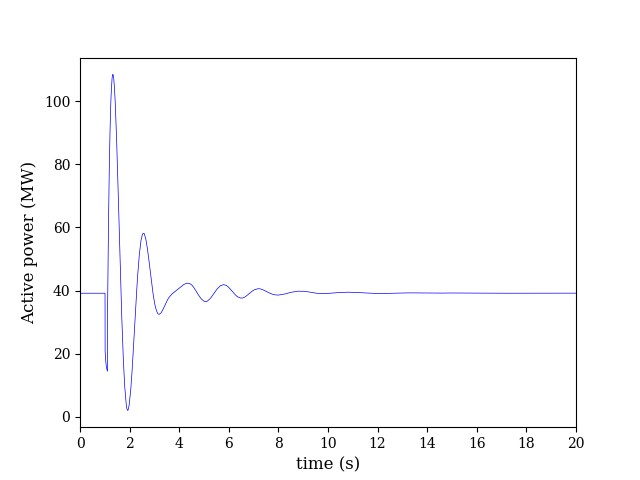
\includegraphics[width=0.49\textwidth]{NodeFault - g2 - P.png}}
    \subfigure[]{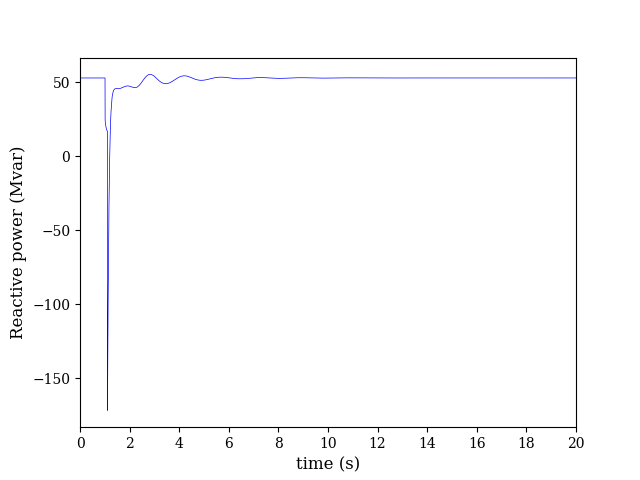
\includegraphics[width=0.49\textwidth]{NodeFault - g2 - Q.png}}
    \subfigure[]{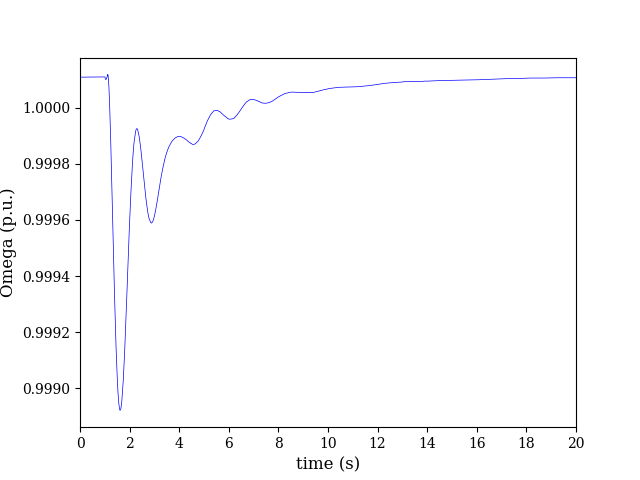
\includegraphics[width=0.49\textwidth]{NodeFault - g2 - omega.png}}
    \subfigure[]{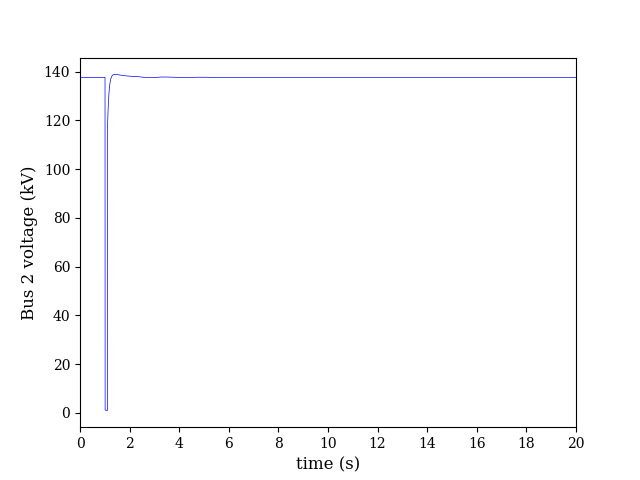
\includegraphics[width=0.49\textwidth]{NodeFault - bus 2 - voltage.png}}
    \caption{Generator 2 response to three-phase fault}
\end{figure}

Generator 1 is electrically close to generator 2. Therefore, when the fault is applied at bus 2, the reactive power injection of generator 1 contributes to limit the voltage dip on bus 1. The active power injection of generator 1 increases to compensate the null injection coming from generator 2 and after the fault clears, oscillates about 8 seconds before returning to its initial value.

\begin{figure}[H]
  \centering
    \subfigure[]{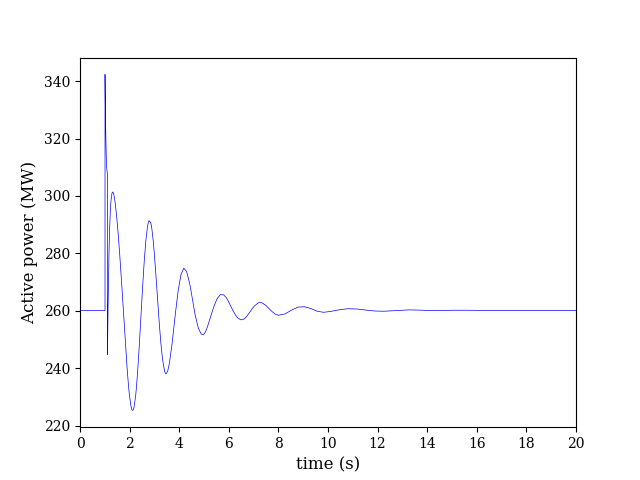
\includegraphics[width=0.49\textwidth]{NodeFault - g1 - P.png}}
    \subfigure[]{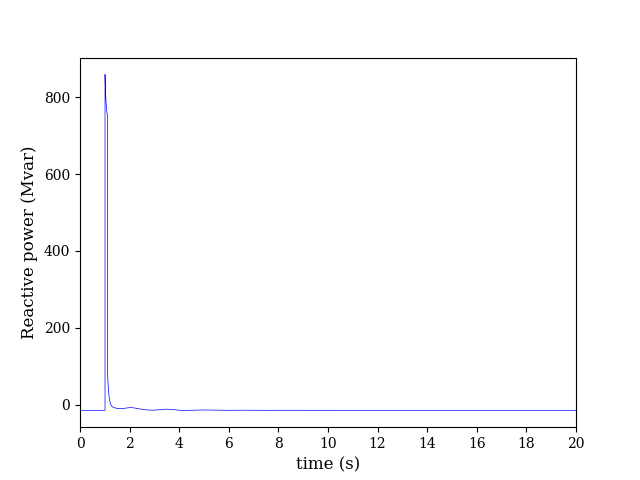
\includegraphics[width=0.49\textwidth]{NodeFault - g1 - Q.png}}
    \subfigure[]{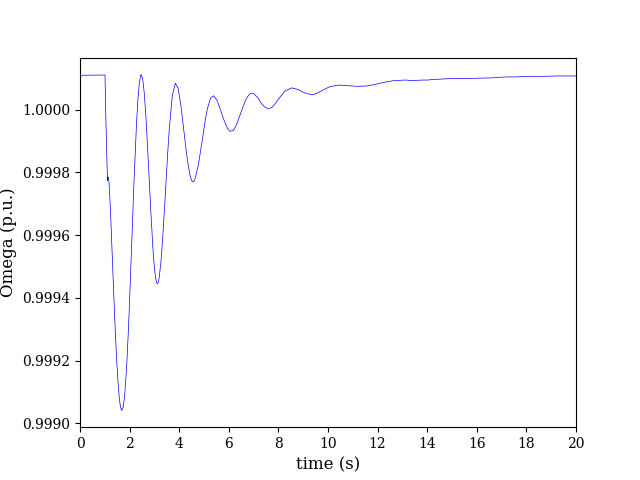
\includegraphics[width=0.49\textwidth]{NodeFault - g1 - omega.png}}
    \subfigure[]{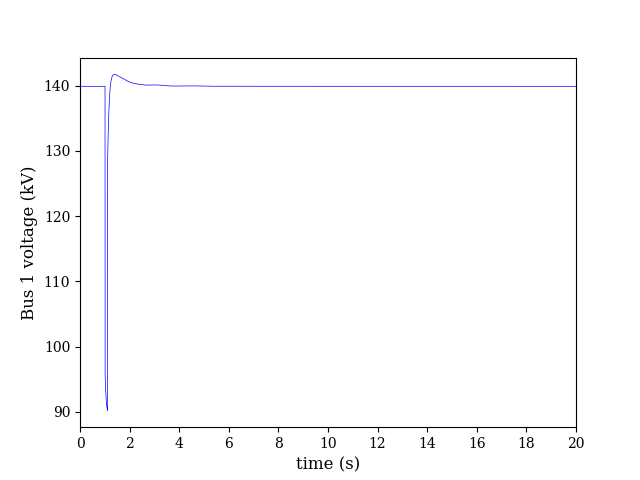
\includegraphics[width=0.49\textwidth]{NodeFault - bus 1 - voltage.png}}
    \caption{Generator 1 response to three-phase fault}
\end{figure}

\chapter{Scenario 2 : Disconnection of line between bus 2 and bus 5}

The simulated scenario is the disconnection of the line between bus 2 and bus 5.

\section{Models}

\begin{itemize}
  \item Generators : GeneratorPV
  \item Loads: restorative loads
\end{itemize}

\section{Solver}

IDA : order 2, absolute accuracy $10^{-4}$, relative accuracy $10^{-4}$. Fixed Backward-Euler order 1 solver with high time step is enough.

\section{Results}

Final values obtained for each generator : \\

\begin{tabular}{ | m{2cm} | m{2cm}| m{2cm} | m{2cm} | m{2cm} | }
  \hline
  \textbf{Generator} & \textbf{P (MW)} & \textbf{Q (Mvar)} & \textbf{U (kV)} & \textbf{$\Theta$ (°)} \\
  \hline
  1 & 263.92 & -12.99 & 139.20 & 0.00 \\
  \hline
  2 & 42.18 & 29.5 & 137.69 & -4.77 \\
  \hline
  5 & 2.18 & 72.46 & 133.32 & -28.05 \\
  \hline
  8 & 2.02 & 40.13 & 133.32 & -15.12 \\
  \hline
  11 & 2.01 & 24.00 & 11.86 & -14.18 \\
  \hline
  13 & 2.06 & 23.24 & 11.78 & -18.47 \\
  \hline
\end{tabular} \\

\pagebreak

And the final power flows on some of the system lines : \\

\begin{tabular}{ | m{2.5cm} | m{2.5cm}| m{2.5cm} | m{2.5cm} | m{2.5cm} | }
  \hline
  \textbf{Line} & \textbf{$P_{Or}$ (MW)} & \textbf{$P_{Ex}$ (MW)} & \textbf{$Q_{Or}$ (Mvar)} & \textbf{$Q_{Ex}$ (Mvar)} \\
  \hline
  Bus1-Bus2 & 155.08 & -150.09 & -17.02 & 23.58 \\
  \hline
  Bus1-Bus3 & 108.74 & -103.19 & 4.04 & 8.99 \\
  \hline
  Bus2-Bus4 & 72.97 & -70.18 & -0.91 & 5.54 \\
  \hline
  Bus2-Bus6 & 98.54 & -93.35 & -5.91 & 17.73 \\
  \hline
  Bus6-Bus28 & 19.62 & -19.56 & -0.35 & -0.74 \\
  \hline
  Bus8-Bus28 & 0.45 & -0.44 & 1.86 & -6.16 \\
  \hline
  Bus10-Bus17 & -0.04 & 0.04 & 1.74 & -1.73 \\
  \hline
  Bus5-Bus7 & -92.01 & 97.17 & 53.46 & -42.52 \\
  \hline
  Bus19-Bus20 & -3.53 & 3.54 & -1.63 & 1.64 \\
  \hline
  Bus23-Bus24 & 4.06 & -4.04 & 2.25 & -2.20 \\
  \hline
  Bus14-Bus15 & 2.79 & -2.77 & 0.98 & -0.96 \\
  \hline
\end{tabular} \\

\chapter{Scenario 3 : Disconnection of generator 2}

The simulated scenario is a disconnection of the generator 2 at t = 50 s.

\section{Models}

\begin{itemize}
  \item Generators : four windings synchronous generators with a proportional voltage regulator and a proportional speed governor. Saturations are considered.
  \item Frequency model: explicit frequency model OmegaRef using different generator speeds
  \item Loads: voltage-dependent loads equipped with tap-changers. The loads connected at 132 kV buses are behind two transformers, while the rest are connected behind one transformer.
\end{itemize}

\section{Solver}

Fixed Backward-Euler order 1 solver, timestep = 1 s, tolerance = $10^{-4}$.

\section{Results}

As a consequence of the generator disconnection, the voltage decreases on the entire network. The voltages at buses 1, 2 and 5 are presented.

\begin{figure}[H]
  \centering
    \subfigure[]{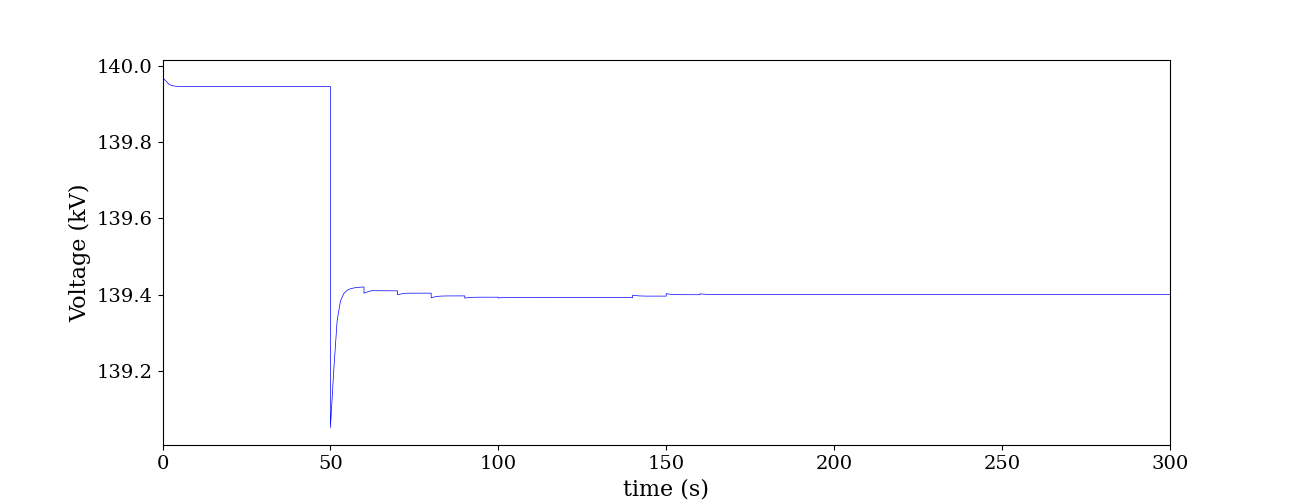
\includegraphics[width=1\textwidth]{DisconnectGroup - bus 1 - voltage.png}}
    \caption{Voltage on bus 1 (kV)}
    \subfigure[]{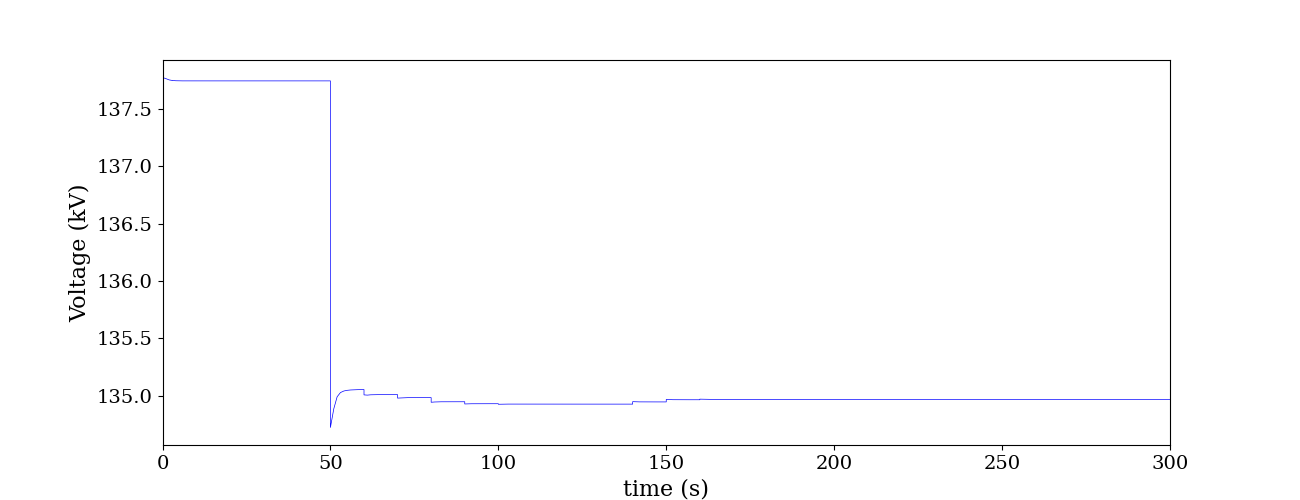
\includegraphics[width=1\textwidth]{DisconnectGroup - bus 2 - voltage.png}}
    \caption{Voltage on bus 2 (kV)}
    \subfigure[]{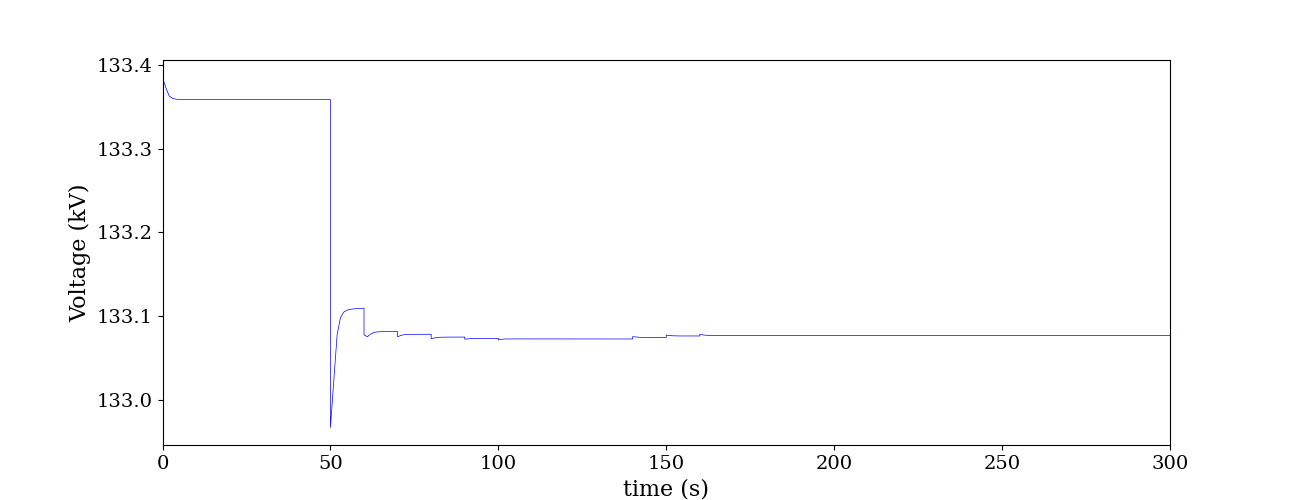
\includegraphics[width=1\textwidth]{DisconnectGroup - bus 5 - voltage.png}}
    \caption{Voltage on bus 5 (kV)}
\end{figure}

\end{document}
